\subsection{E8 --- Objection 3: where should each read run? Computation placement under contention}
\label{sec:e8}
\textbf{Question.} E1--E7 chose where data live, and the tier implied where a read was computed, with latencies summed serially. A memory-centric design must also decide \emph{where the computation runs} when compute units are finite and share a data path. Does the compute-site decision matter, and does the data-placement result survive contention? \textbf{Setup.} The system model of Sec.~\ref{sec:sys}, dense (reusable) reads, 42 traces on SmolVLM-256M. Policies: flat, static modality, and the dynamic policy at the E5 thresholds ($8\times/0.4\times$, \emph{not} re-tuned) with the bottom-up migration cost. Schedulers: \texttt{tier} (\warm{} reads run in memory), \texttt{host} (\warm{} is compressed storage; every read runs on the host) and \texttt{adaptive}. CIM capacity is swept from 2 to 64 units; 8 bus channels and 8 host lanes are fixed. Hypotheses and pass criteria H8a--H8c were written in the lab notes after the runs were launched but before any result was inspected (apart from one smoke-test trace). Values are means over traces of per-trace ratios to flat (the trace-to-trace s.d.\ of every ratio is below 0.01 for energy and below 0.04 for makespan).

\begin{figure}[t]
\centering
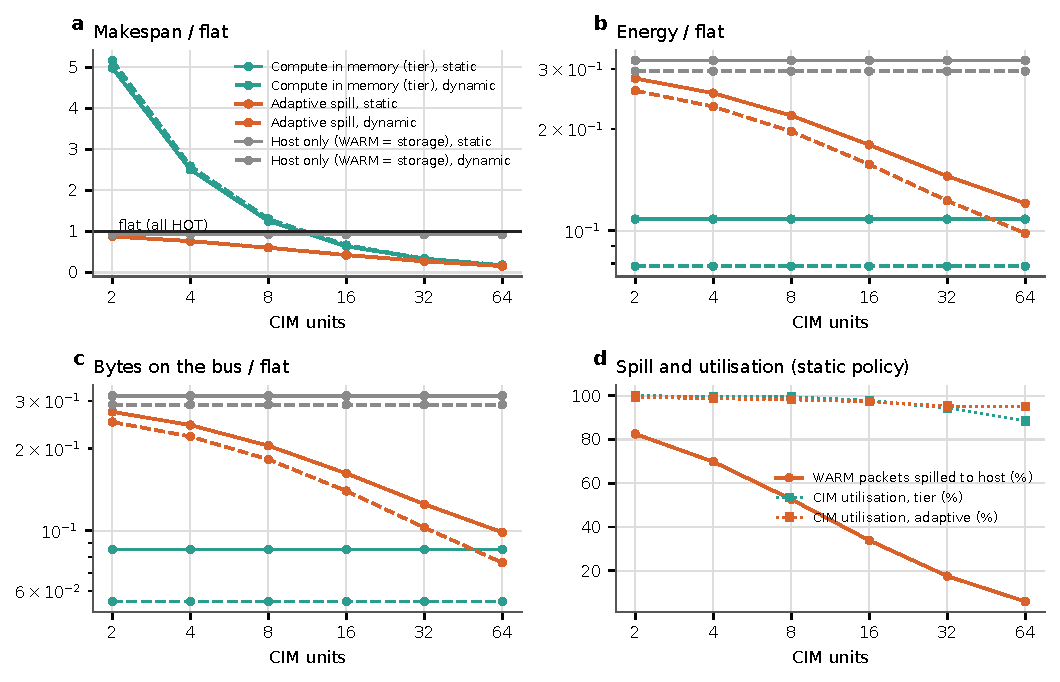
\includegraphics[width=\linewidth]{figs/fig_e8.pdf}
\caption{E8: compute-site scheduling vs CIM capacity (dense reads, 42 traces; solid = static modality, dashed = dynamic). (a) Makespan relative to flat: compute-in-memory alone is slower than flat below $\sim$16 units; host-only is capacity-independent; adaptive spill beats both. (b) Energy and (c) bytes on the bus relative to flat. (d) Fraction of \warm{} packets the adaptive scheduler spills to the host, and CIM utilisation.}
\label{fig:e8}
\end{figure}

\textbf{H8a --- contention reverses the serial-latency penalty: confirmed.} With 16 CIM units, static modality moves $11.8\times$ fewer bytes over the bus than flat, uses $9.3\times$ less energy and has a \emph{lower} makespan ($0.64\times$ flat's). Flat is bus-bound (99\% bus utilisation); static modality is CIM-bound (98\%). In the serialised model of E1--E7 the same placement looked $\sim$34\% \emph{slower} than flat, because serialisation forbids overlapping the two tiers. Part of what E1--E7 called a latency cost of tiering was an artefact of the cost model.

\textbf{H8b --- the compute-site decision is first-order: confirmed.} If \warm{} reads always run in memory, the verdict depends on CIM capacity: static modality is $5.0\times$, $2.5\times$ and $1.25\times$ \emph{slower} than flat with 2, 4 and 8 units, and breaks even near 16 (Fig.~\ref{fig:e8}a). The opposite extreme, treating \warm{} as compressed storage computed on the host, is capacity-independent ($0.92\times$ flat's makespan) but gives up most of the benefit: energy $0.319$ of flat versus $0.108$, and bytes on the bus $0.313$ versus $0.085$ (Fig.~\ref{fig:e8}b,c). The adaptive scheduler is better on makespan than \emph{both} at every capacity (e.g.\ $0.42\times$ flat at 16 units, against $0.64\times$ and $0.92\times$), because it keeps the CIM units and the host lanes busy at once; it spills 83\% of \warm{} packets at 2 units and 6\% at 64 (Fig.~\ref{fig:e8}d). The price is energy: at 16 units adaptive uses $1.66\times$ the energy of in-memory compute ($0.179$ vs $0.108$ of flat) for a $33\%$ lower makespan, still far below host-only ($0.319$). Compute placement is therefore a latency--energy trade-off that the runtime resolves from queue state, not a property of the tier.

\textbf{H8c --- data-placement gains survive contention: confirmed, with a latency cost.} At 16 CIM units with in-memory compute, the dynamic policy lowers energy by \textbf{27.4\%} against static modality (95\% CI $[27.0,27.8]$; larger than E5's $-22.3\%$ because the bottom-up migration costs $\approx\!1.05$ rather than $10$ \hot{} accesses) and bytes on the bus by $36\%$, at quality $2.5\%$ better. It is $4.7\%$ ($[4.6,4.9]$) \emph{slower} in makespan, plausibly because it keeps more entries on the host-side path and its 1.1k moves per session compete for the bus (we did not isolate the two). Under the adaptive scheduler the energy advantage over static shrinks to $12.5\%$ at 16 units and to $8.0\%$ at 2: spilled reads cost the same on the host regardless of how \warm{} came to hold the data, so a scarce CIM tier dilutes what any tiering policy can save.

\textbf{What E8 left open.} All of E1--E8 read every entry every step (or the top-$k$ of it). The task statement's own example has data with different \emph{reuse}: re-read, streamed once, accessed at random. E9 tests whether placement should differ across them.
